\chapter{RIK model}
\label{chapRIK}


RIK (Ruiz's Integral Kinematic) model is an advanced kinematic source model developed by \cite{Ruiz2011} and further modified by \cite{Gallovic2016}. This method allows taking into account frequency-dependent directivity effects. The asperities have a fractal distribution that may follow a given inverted slip distribution. \\


The kinematic source model could be generated by using the RIKsrf code. It is provided in RIK\textunderscore MODEL/CODE\textunderscore GALLOVIC\textunderscore RIKsrf/ folder of the materials of this manual. Its compilation is verified for gfortran and ifort compilers. Two different sub-folders are available depending on compiler selection. Inside the selected sub-folder, the user should just run 'lancer.sh' file in order to compile the code, which creates the executable 'RIKsrf2'. \\ 


RIKsrf code works by calling the executable RIKsrf2 from any example folder. In this manual, a case from South Napa fault model is used as an example. The related folder to this example is 'RIK\textunderscore MODEL/EXAMPLES/NAPA\textunderscore ROCHER/'. Two input files are needed to run the RIKsrf code. The first one is 'RIKsrf.in'. The 'RIKsrf.in' file for Napa example is shown in the figure below:


%% FIGURE : RIKsrf.in
\begin{center}
\leavevmode
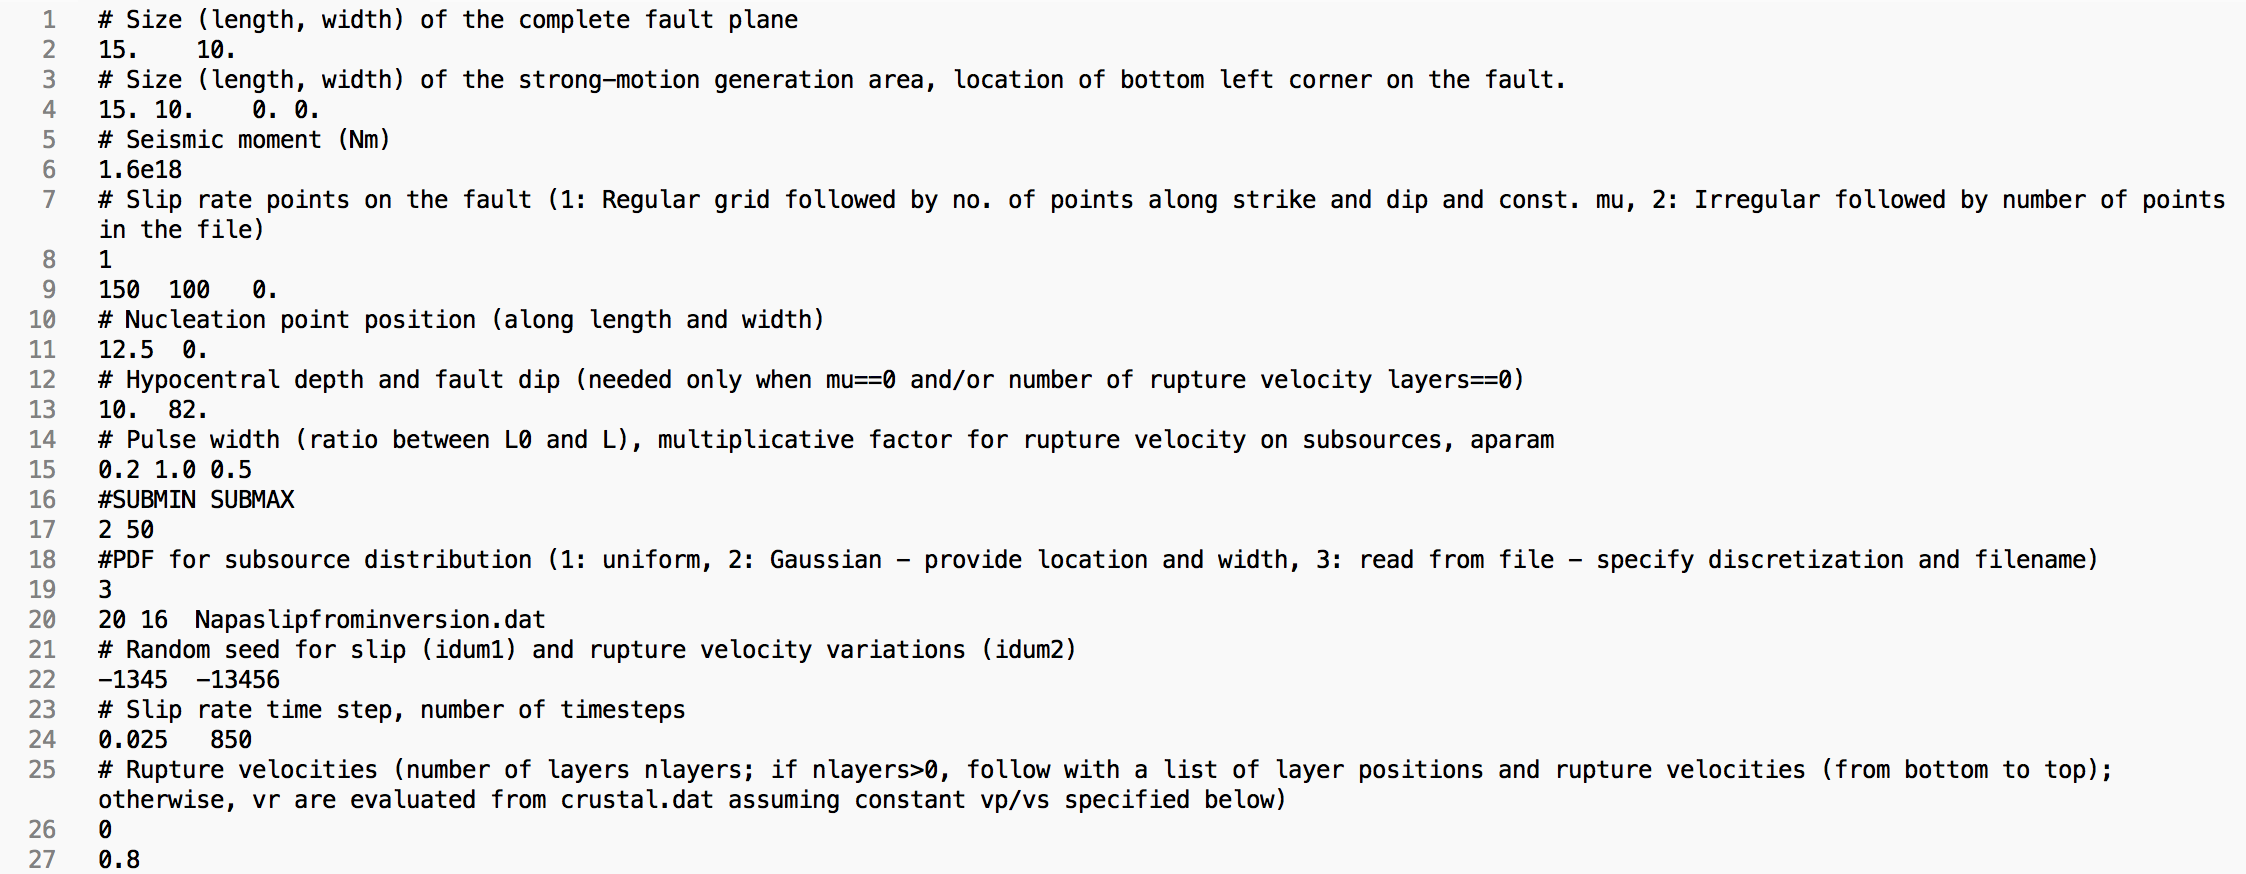
\includegraphics[scale=0.45]{figures/RIK-input1.png} 
\captionof{figure}{RIKsrf.in file for RIK model}
\label{rik1} 
\vspace{1cm}
\end{center}



In line 2, we define the size of fault plan (length and width). For our example, length is equal to 15 km and width is 10 km. The strong-motion generation area is the same as the complete fault plan. Thus, in line 4, we enter 15 and 10 for strong-motion generation area and the location of left bottom point. \\

In line 6, seismic moment is given in Nm. \\

In lines 8-9, we specify the choice of grid model. If a regular model is desired, 1 is written in line 8 and followed by the point number along strike and dip. Otherwise, the grid is determined by a given file. In our example, we work with a regular grid. In line 9, after point numbers, a constant rigidity value is specified. Since it is not used in this example, we write 0.  \\

In line 11, we define the location of hypocenter in fault plan. In our test, it is located at (12.5, 0). \\


In line 13, hypocenter depth and dip angle are written. \\


In line 15, impulse characteristics are defined based on \cite{Ruiz2011} model. For more details, please refer to \cite{Ruiz2011} and \cite{Gallovic2016}. \\


In line 17, the upper and lower limits that determine the size-distribution of asperities (sub-sources) are defined. \\

In lines 19-20, we specify the choice of slip-inversion data. In our example, we provide inverted slip distribution for Napa model so that in line 19 we enter 1 and in line 20 the file name is given. \\


In line 22, random seed for slip and rupture velocities are set. \\

In line 24, the time step and total duration for slip-velocity time histories are specified. \\

Lastly, in line 26, we define rupture velocities of layers in the model. Either one line is devoted to the property of each layer either it is provided by another file named 'crustal.dat'. In our case, we give another file. For such cases where 'crustal.dat' is used, a constant value (0.8 in this example) is set for rupture-to-shear velocity ratio. \\


In the following, we explain the content of 'crustal.dat' file in our example, Figure \ref{rik2}.



%% FIGURE : RIKsrf.in
\begin{center}
\leavevmode
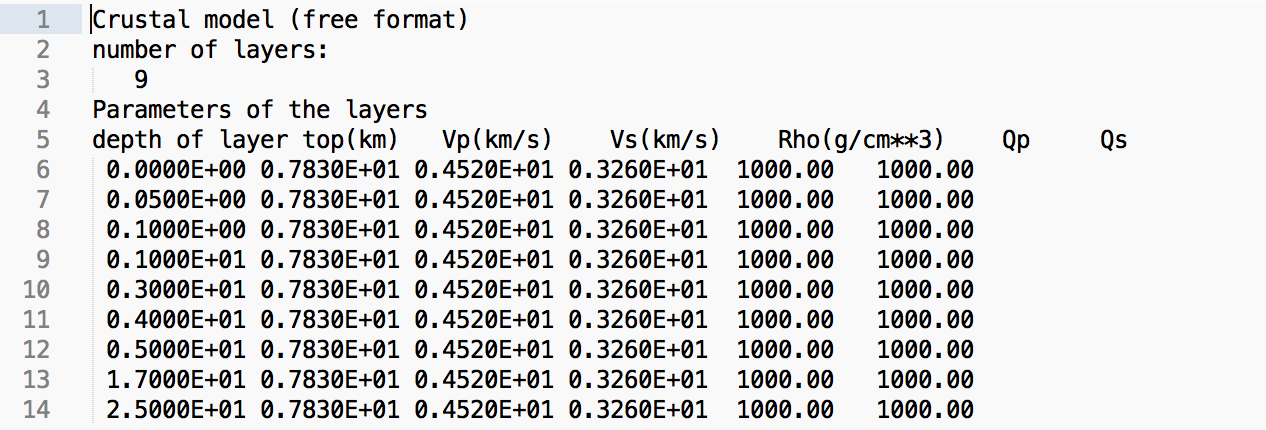
\includegraphics[scale=0.45]{figures/RIK-input2.png} 
\captionof{figure}{crustal.dat file for RIK model}
\label{rik2} 
\vspace{1cm}
\end{center}



First, in line 3, total number of layers is given. Then, starting from line 6, for each layer in the model, the depth of top level (positive in downward), pressure and shear wave velocities, density and quality factors for pressure and shear waves are defined. \\


After the simulation, the code sorts a number of output files such as slipdistribution.dat, subsources.dat etc. In RIK\textunderscore MODEL/EXAMPLES/python folder, two Python scripts are provided to plot maximum-slip distribution and asperity distribution on fault plan (slip.py and subsources.py respectively). For our example, the resultant figures for maximum-slip distribution and asperity distribution are given in Figures \ref{rik3}-\ref{rik4}.\\




%% FIGURE : RIKsrf.in
\begin{center}
\leavevmode
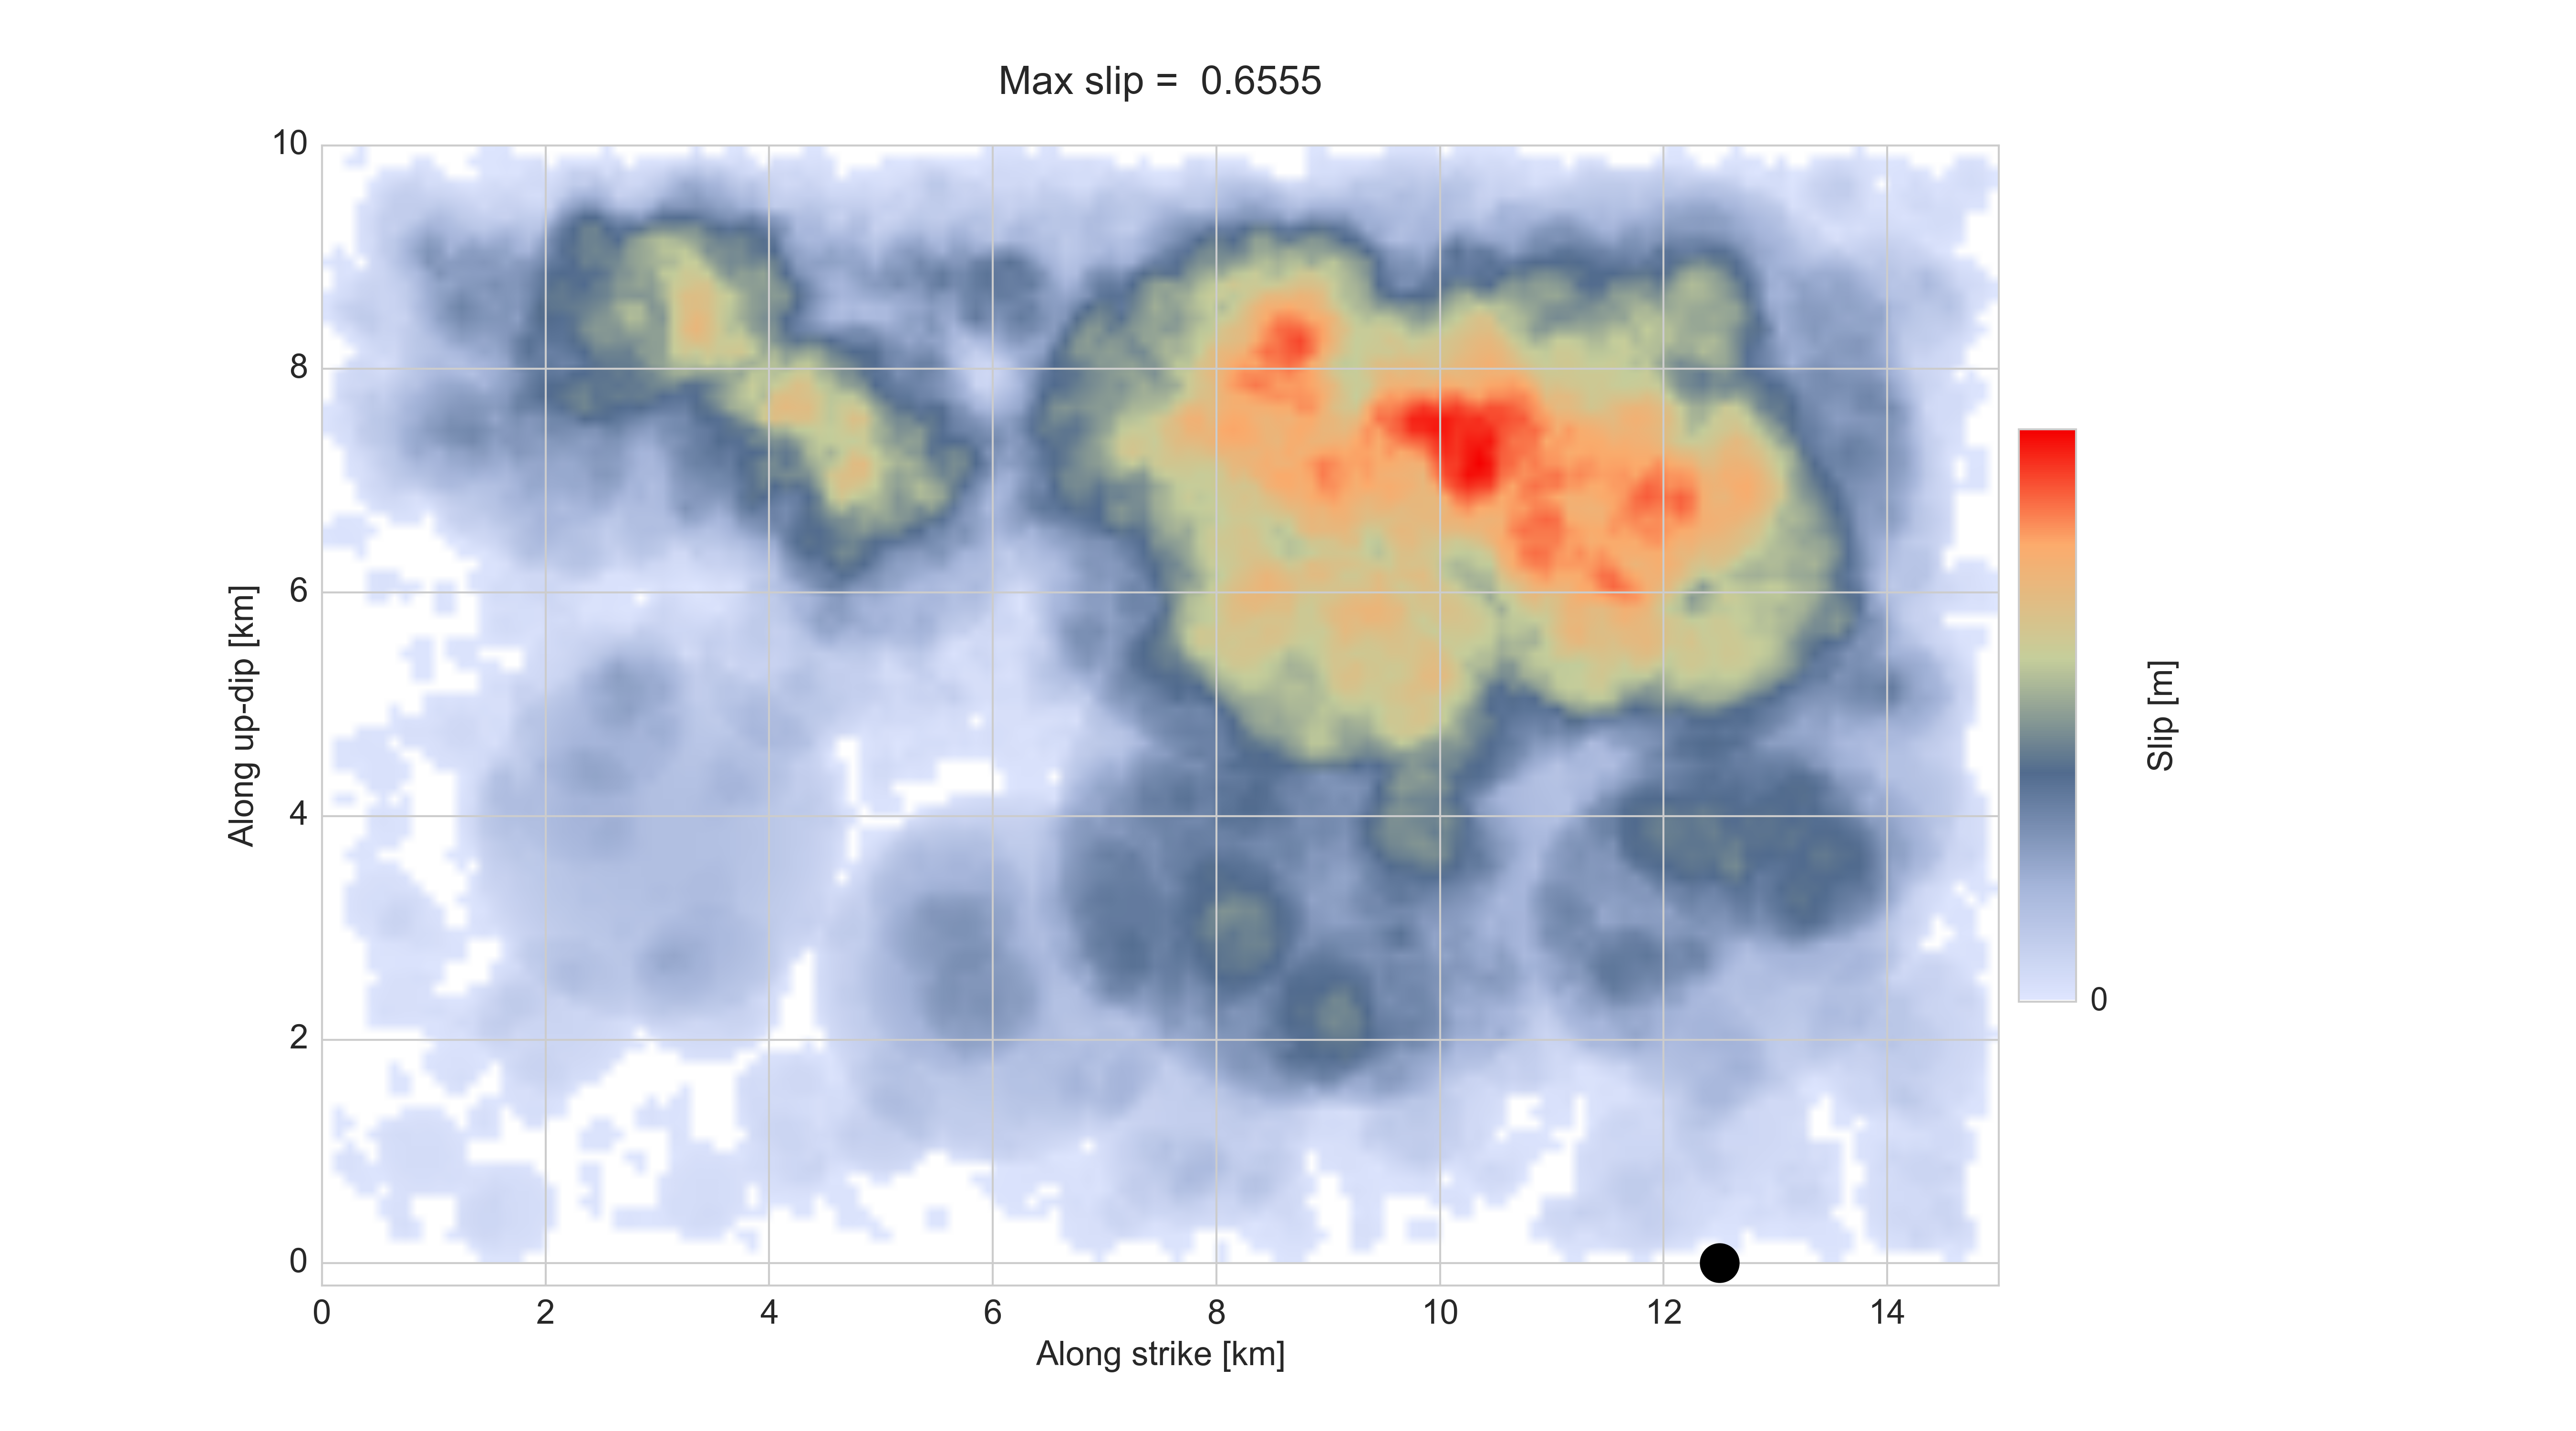
\includegraphics[scale=0.35]{figures/15000points_Napa_rocher_slip.png} 
\captionof{figure}{Maximum-slip distribution on fault plan of Napa event.}
\label{rik3} 
\vspace{1cm}
\end{center}




%% FIGURE : RIKsrf.in
\begin{center}
\leavevmode
\includegraphics[scale=0.35]{figures/15000points_Napa_rocher_circles.png} 
\captionof{figure}{Asperity distribution on fault plan of Napa event.}
\label{rik4} 
\vspace{1cm}
\end{center}













 